\documentclass[conference]{IEEEtran}
\IEEEoverridecommandlockouts
% The preceding line is only needed to identify funding in the first footnote. If that is unneeded, please comment it out.
\usepackage[ngerman]{babel}
\usepackage{cite}
\usepackage{amsmath,amssymb,amsfonts,mathtools}
\usepackage{algorithmic}
\usepackage{graphicx}
\usepackage{textcomp}
\usepackage[dvipsnames]{xcolor}
\def\BibTeX{{\rm B\kern-.05em{\sc i\kern-.025em b}\kern-.08em
    T\kern-.1667em\lower.7ex\hbox{E}\kern-.125emX}}
\usepackage{listings}
\usepackage{tabularx}
\usepackage{booktabs}
\usepackage{siunitx}
\usepackage{float}
\usepackage{caption}

\definecolor{codegreen}{rgb}{0,0.6,0}
\definecolor{codegray}{rgb}{0.5,0.5,0.5}
\definecolor{codepurple}{rgb}{0.58,0,0.82}
\definecolor{backcolour}{rgb}{0.95,0.95,0.95}
\renewcommand{\lstlistingname}{Code}% Listing -> Algorithm
\renewcommand{\lstlistlistingname}{List of \lstlistingname s}% List of Listings -> List of Algorithms
\lstdefinestyle{mystyle}{
    backgroundcolor=\color{backcolour},
    commentstyle=\color{codegreen},
    keywordstyle=\color{magenta},
    numberstyle=\tiny\color{codegray},
    stringstyle=\color{codepurple},
    basicstyle=\ttfamily\footnotesize,
    breakatwhitespace=false,
    breaklines=true,
    captionpos=b,
    keepspaces=true,
    numbers=left,
    numbersep=3pt,
    showspaces=false,
    showstringspaces=false,
    showtabs=false,
    tabsize=3
}
\lstset{style=mystyle}

\usepackage{hyperref}
\hypersetup{
    pdftex,
    pdftitle={Versuch ASM},
    pdfsubject={Versuch ASM},
    pdfauthor=AJC,
    colorlinks,
    citecolor=black,
    filecolor=black,
    linkcolor=black,
    urlcolor=black
}



\begin{document}

\title{
    \centering
    
\includegraphics[width=0.5\textwidth]{../OTHR_OTHR_Logo.pdf}\\
    \textsc{Drehstrom-Asynchronmaschine mit Schleifringläufer} \\
}

\maketitle

\begin{abstract}
    In diesem Versuch soll eine Käfigläufer-Asynchronmaschine genauer
    untersucht werden. Zur Bestimmung der ESB- Parameter wurde hierzu der
    Leerlauf, als auch Kurzschlussversuch durchgeführt\dots
\end{abstract}

\section{Anlaufmoment und Kippmoment}

Bei diesem Versuch wurde das Drehmoment mit einem 40cm langen Stab und einer
Digitalen Wage gemessen.

Mit der Gleichung \ref{eq:moment} wurde das Drehmoment aus den Messungen berechnet.

\begin{equation} \label{eq:moment}
    M=G\cdot g\cdot l = \frac{G(I_1)}{1000}\si{kg}\cdot 9.81\si{m/s^2} \cdot 0.4\si{m}
\end{equation}

In den Abbildungen \ref{fig:Anlaufmoment} und \ref{fig:Kippmoment} wird das
Anlaufmoment der ASM über die Spannung graphisch dargestellt.

Die obere Hälfte der Abbildungen zeigt eine linearisierte Extrapolation des
Verlaufs der Drehmomente $M_{an}$ und $M_{\textit{Kipp}}$ über die Spannung
$U_1^2$, bis $400^2V$.

Aber in der unteren Hälfte der Abbildungen wird das Drehmoment der ASM direkt
über die Spannung $U_1$ dargestellt und mit einer quadratischen Polynomfunktion
extrapoliert.

\vspace{-7ex}
\begin{figure}[htbp]
    \centering
    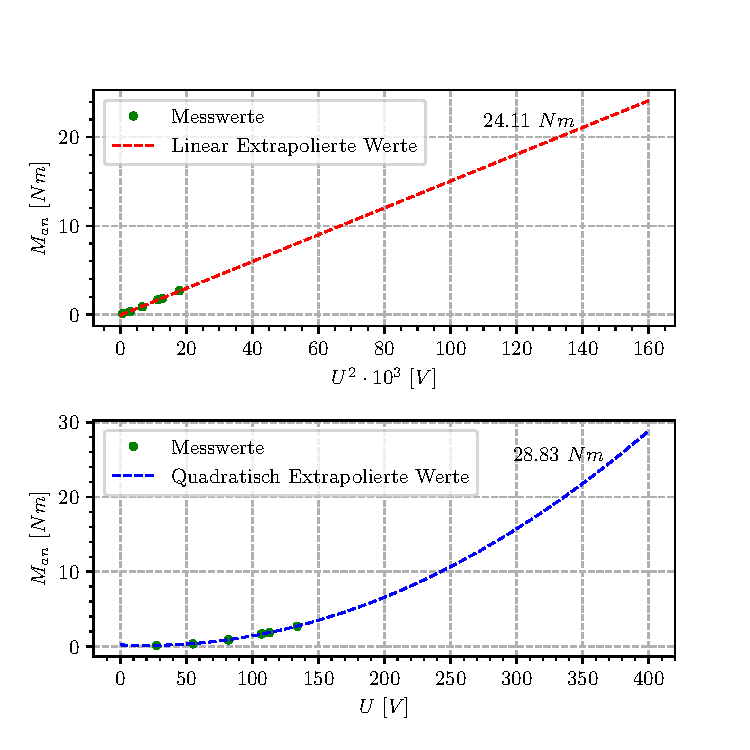
\includegraphics[width=\columnwidth]{./anlaufmoment.pdf}
    \caption{Anlaufmoment}
    \label{fig:Anlaufmoment}
\end{figure}

Der lineare Verlauf in Abb.\ref{fig:Anlaufmoment}, $M_{an}(U)$ [\textcolor{red}{rot}]:
\begin{gather*}
    0,1511 x - 0,07306 \\
    M_{an}(U_N=400^2V^2)=24,11\ \si{Nm}
\end{gather*}

Und die quadratische Polynomfunktion $M_{an}(U)$ [\textcolor{blue}{blau}]:
\begin{gather*}
    0,000199 x^2 -0,007889 x + 0,190977\\
    M_{an}(U_N=400V)=28,83\ \si{Nm}
\end{gather*}

\vspace{-7ex}
\begin{figure}[htbp]
    \centering
    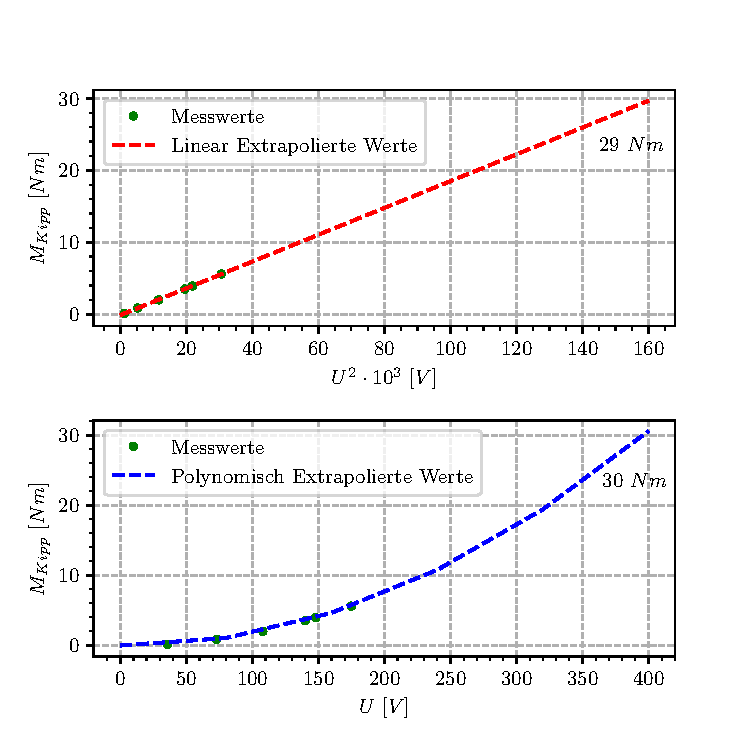
\includegraphics[width=\columnwidth]{./kippmoment.pdf}
    \caption{Kippmoment}
    \label{fig:Kippmoment}
\end{figure}

Der lineare Verlauf in Abb.\ref{fig:Kippmoment}, $M_{\textit{Kipp}}(U)$ [\textcolor{red}{rot}]:
\begin{gather*}
    0,1863 x - 0,1431\\
    M_{Kipp}(U_N=400^2V^2)=29,67 \ \si{Nm}
\end{gather*}

Und die quadratische Polynomfunktion $M_{\textit{Kipp}}(U)$ [\textcolor{blue}{blau}]:
\begin{gather*}
    0,000198 x^2 - 0,0024495 x -0,035842\\
    M_{Kipp}(U_N=400V)=30,6\ \si{Nm}
\end{gather*}



\subsection{Zusammenhang zwischen Drehmoment und Spannung}

Bei zunehmender Spannung $U_1$ steigt das Drehmoment M quadratisch an. Das
Drehmoment ist direkt proportional zu $U^2$ ($M \sim U^2$) und darauf ergibt sich
folgende Beziehnung: \[ M = \textit{konst.} \cdot U \]


\section{Bestimmung der Ersatzschaltbildparameter}
\subsection{Parameterbestimmung aufgrund der Kurzschlussmessung}

Umrechnen der gemessenen Widerstandswerte auf die Bezugstemperatur $T=75^\circ$C :
\begin{align*}
    R_{1_{75}} & = R_{1_{20}}\frac{235^\circ\si{C}+75^\circ\text{C}}{235^\circ\text{C}+20^\circ\text{C}}         \\
               & = 2,32\ \Omega\cdot \frac{235^\circ\si{C}+75^\circ\text{C}}{235^\circ\text{C}+20^\circ\text{C}} \\
               & = 2,820\ \Omega
\end{align*}

Berechnen des Läuferwiderstands mithilfe der Übersetzungsverhältnis:
\begin{align*}
    R_2^\text{\textquotesingle}        & = \ddot{u}^2\cdot R_2 = 4,7^2 \cdot 216\si{m\Omega}   = 4,77 \Omega                             \\
    R_{2_{75}}^\text{\textquotesingle} & = R_{2_{20}}\frac{235^\circ\si{C}+75^\circ\text{C}}{235^\circ\text{C}+20^\circ\text{C}}         \\
                                       & = 4,77\ \Omega\cdot \frac{235^\circ\si{C}+75^\circ\text{C}}{235^\circ\text{C}+20^\circ\text{C}} \\
                                       & = 5,8\ \Omega
\end{align*}

Es gilt:
\begin{equation} \label{eq:Kurzschlusswiderstand_gemessen}
    \boxed{R_k = R_1 + R_2^\text{\textquotesingle} = 2,820\ \Omega + 5,8\ \Omega = 8,62\ \Omega}
\end{equation}

Aus der Kurzschlussmessung in 4.2.1 wird der Kurzschlusswiderstand $R_k$ mit:

\begin{equation}
    \boxed{R_k = \frac{U_k}{I_k}\cdot cos\varphi_k}
\end{equation}

\begin{table}[htbp]
    \begin{tabularx}{\columnwidth}{XXXXX}
        \toprule
        $I_1[A]$ & $P_1[W]$ & $U[V]$ & $G[g]$ & $M_{an}[Nm]$ \\
        \midrule
        4,2      & 392      & 113    & 464    & 1,82074      \\
        \bottomrule
    \end{tabularx}
    \caption{Kurzschlussmessung 4.2.1}
    \label{tab:Kurzschlussmessung}
\end{table}

Mit den Werten aus der Tabelle \ref{tab:Kurzschlussmessung} kann $cos\varphi_k$ berechnet werden:

\begin{equation}
    \boxed{cos\varphi_k = \frac{P_1}{\sqrt{3} \cdot I_1 \cdot U}}
\end{equation}

\begin{equation} \label{eq:cosphi_solved}
    cos\varphi_k = \frac{392 \si{W}}{\sqrt{3} \cdot 4,2 \si{A} \cdot 113 \si{V}} = 0,4769
\end{equation}

Da die Maschine im Stern geschaltet ist, ergibt sich für die Spannung $U_k$:

\begin{equation} \label{eq:Uk_solved}
    \boxed{U_k = \frac{U}{\sqrt{3}}} = \frac{113 \si{V}}{\sqrt{3}} = 65,24 \si{V}
\end{equation}

Jetzt kann $R_k$ aus den Formeln \ref{eq:Ik_solved_real} und \ref{eq:Uk_solved} berechnet werden:

\begin{equation} \label{eq:Kurzschlusswiderstand_calc}
    \boxed{R_k = \frac{65,24\si{V}}{4,2\si{A}}\cdot cos(61,51^\circ) = \underline{7,409 \Omega}}
\end{equation}

Die Streureaktanzen $X_{1\sigma}$ und $X_{2\sigma}^\text{\textquotesingle}$ werden mit:

\begin{equation} \label{eq:Streureaktanzen}
    X_{1\sigma} + X_{2\sigma}^\text{\textquotesingle} = \frac{U_k}{I_k}\cdot sin\varphi_k
\end{equation}

Da $X_{1\sigma} = X_{2\sigma}^\text{\textquotesingle}$ ist, ergibt sich:

\begin{align} \label{eq:Streureaktanzen_solved}
    \Aboxed{X_{1\sigma} & = X_{2\sigma}^\text{\textquotesingle} = \frac{U_k}{I_k}\cdot\frac{1}{2}\cdot sin\varphi_k} \\
                        & = \frac{65,24\si{V}}{3,69\si{A}}\cdot\frac{1}{2}\cdot sin(61,51^\circ)   \\
                        & =6,826\ \Omega
\end{align}

\subsubsection{Vergleich zwischen ermittelter und gemessener Kurzschlusswiderstand}

Die Werte der Widerstände liegen nah beieinander. Der kleine Differenz kann
durch Messunsicherheiten begründet werden (Analoge Messgeräte).

\section{Trennung von Eisen- und Reibungsverlusten}
\begin{figure}[htbp]
    \centering
    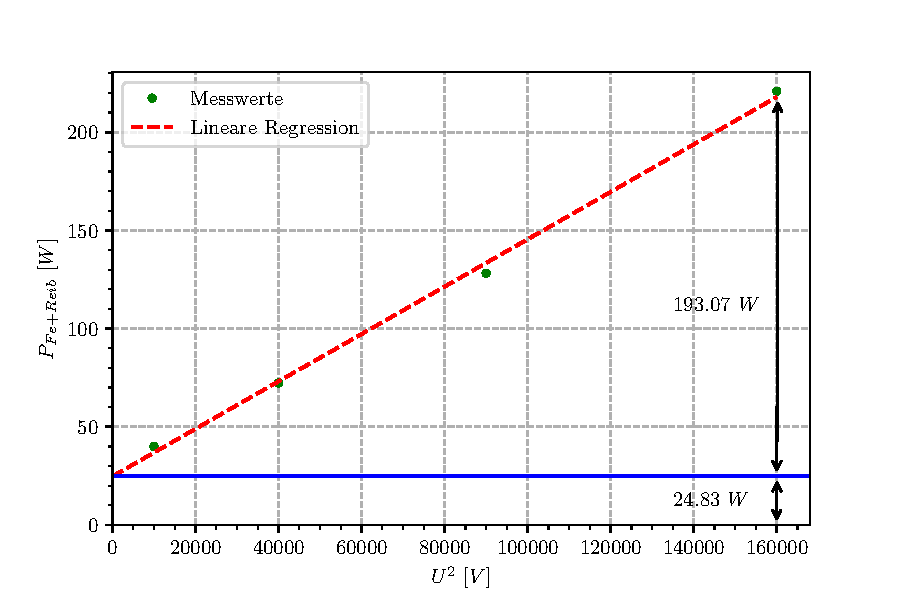
\includegraphics[width=\columnwidth]{./trennung_eisen_reib.pdf}
    \caption{Trennung von Eisen- und Reibungsverlusten}
    \label{fig:trennung_von_eisen_reib}
\end{figure}

\end{document}
